Data will be recorded uses the LEAP motion, a commercial technology that captures precise data about the hands.
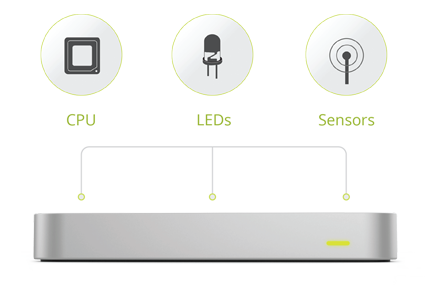
\includegraphics[width=\columnwidth]{images/leap.jpg}
The LEAP Motion plugs into computers via USB and sends information about any hands it sees in its field of view, which is a cone of about 8 cubic feet above it.
It then determines the location of fingers within the field of view, the angle of the hand, the existence and position of any "tools," such as pens or pencils, and an approximation of the curvature of the palm.
This paper only uses the finger  and tool position data taken from the LEAP motion. The LEAP can capture these finger points at approximately 100 fps using USB 2.0 port or about 150 using a USB 3.0 port.
The importance of this type of input devices is that when the user is writing, there is no explicit "beginning" and "end" of writing. There is no predefined gesture that defines when writing characters begins and ends. Instead, this input device would require that the entire stream of data points be searched for instances of letters. 
